% ******************************* PhD Thesis Template **************************
% Please have a look at the README.md file for info on how to use the template

\documentclass[a4paper,12pt,times,numbered,print,index,doublelinesep]{PhDThesisPSnPDF}


\usepackage{import}

\usepackage{paralist}
\usepackage[english]{babel}
\usepackage{cleveref}
\usepackage{xstring}
\usepackage{xcolor}
\usepackage{mdframed}
\usepackage{cleveref}
\usepackage{caption}
\usepackage{subcaption}
\usepackage{amsthm}
% \usepackage{url}
\usepackage{dirtree}
\usepackage{multirow}
\usepackage{array}
\usepackage{textcomp}
\usepackage{gensymb}
\usepackage{siunitx} 
\usepackage{booktabs} 
\usepackage{pgf}
\usepackage{longtable}

%%%%%%%%%%%%%%%%%%%%%%%% extra commands %%%%%%%%%%%%%%%%%% 
%%%%%%%%highlighting 
\newcommand\note[1]{\textcolor{red}{\bf\em{TODO : #1}}}
\newcommand\best[1]{\textcolor{teal}{\bf #1}}
\newcommand\wow[1]{\textcolorcolor{orange}{\em #1}}
\newcommand\yes[0]{\checkmark}
\newcommand\no[0]{--}

\newcommand\fnurl[2]{%
\href{#2}{#1}\footnote{\url{#2}}%
}


\newcommand{\todo}[1]{{\color{red}\bf\em TODO: #1}}
\newcommand{\romain}[1]{{\color{blue}\bf\em Cmt[R]: #1}}
\newcommand{\reference}[1]{{\color{green}\bf\em ADD Reference: #1}}


\newcommand{\expires}{\texttt{Expires}}
%THIS MEANS RECHECK IT, I CHANGED IT.
\newcommand{\hl}[1]{\textcolor{red}{#1}}
%\newcommand{\hl}[1]{#1}
%THIS MEANS PROBLEM, TEXT IS NOT CLEAR.
\newcommand{\hll}[1]{\textcolor{orange}{#1}}
\newcommand{\point}[1]{\par\smallskip\noindent\textbf{#1:}}
\newcommand{\nrange}[4][]{%
  \def\@temp@a{#1}%
  #2=%
  \ifx\@temp@a\@empty
  #3, \dots ,#4%
  \else
  #3, #1, \dots,#4%
  \fi
}
% ******************************************************************************
% ******************************* Class Options ********************************
% *********************** See README for more details **************************
% ******************************************************************************

% `a4paper'(The University of Cambridge PhD thesis guidelines recommends a page
% size a4 - default option) or `a5paper': A5 Paper size is also allowed as per
% the Cambridge University Engineering Deparment guidelines for PhD thesis
%
% `11pt' or `12pt'(default): Font Size 10pt is NOT recommended by the University
% guidelines
%
% `oneside' or `twoside'(default): Printing double side (twoside) or single
% side.
%
% `print': Use `print' for print version with appropriate margins and page
% layout. Leaving the options field blank will activate Online version.
%
% `index': For index at the end of the thesis
%
% `draftclassic': For draft mode without loading any images (same as draft in book)
%
% `draft': Special draft mode with line numbers, images, and water mark with
% timestamp and custom text. Position of the text can also be modified.
%
% `abstract': To generate only the title page and abstract page with
% dissertation title and name, to submit to the Student Registry
%
% `chapter`: This option enables only the specified chapter and it's references
%  Useful for review and corrections.
%
% ************************* Custom Page Margins ********************************
%
% `custommargin`: Use `custommargin' in options to activate custom page margins,
% which can be defined in the preamble.tex. Custom margin will override
% print/online margin setup.
%
% *********************** Choosing the Fonts in Class Options ******************
%
% `times' : Times font with math support. (The Cambridge University guidelines
% recommend using times)
%
% `fourier': Utopia Font with Fourier Math font (Font has to be installed)
%            It's a free font.
%
% `customfont': Use `customfont' option in the document class and load the
% package in the preamble.tex
%
% default or leave empty: `Latin Modern' font will be loaded.
%
% ********************** Choosing the Bibliography style ***********************
%
% `authoryear': For author-year citation eg., Krishna (2013)
%
% `numbered': (Default Option) For numbered and sorted citation e.g., [1,5,2]
%
% `custombib': Define your own bibliography style in the `preamble.tex' file.
%              `\RequirePackage[square, sort, numbers, authoryear]{natbib}'.
%              This can be also used to load biblatex instead of natbib
%              (See Preamble)
%
% **************************** Choosing the Page Style *************************
%
% `default (leave empty)': For Page Numbers in Header (Left Even, Right Odd) and
% Chapter Name in Header (Right Even) and Section Name (Left Odd). Blank Footer.
%
% `PageStyleI': Chapter Name next & Page Number on Even Side (Left Even).
% Section Name & Page Number in Header on Odd Side (Right Odd). Footer is empty.
%
% `PageStyleII': Chapter Name on Even Side (Left Even) in Header. Section Number
% and Section Name in Header on Odd Side (Right Odd). Page numbering in footer

% Uncomment to change page style
%\pagestyle{PageStyleII}

% ********************************** Preamble **********************************
% Preamble: Contains packages and user-defined commands and settings
% \input{Preamble/preamble}

% ************************ Thesis Information & Meta-data **********************
% Thesis title and author information, refernce file for biblatex
% ************************ Thesis Information & Meta-data **********************
%% The title of the thesis
\title{Studying the Impact of Programming~Frameworks on the Energy~Consumption of Software~Services}
%\texorpdfstring is used for PDF metadata. Usage:
%\texorpdfstring{LaTeX_Version}{PDF Version (non-latex)} eg.,
%\texorpdfstring{$sigma$}{sigma}

%% Subtitle (Optional)
% \subtitle{}
\crest{
    
\includegraphics[width=.3\linewidth]{Figs/logo-inria}\,
    
\includegraphics[width=.3\linewidth]{Figs/logo-univ-lille}\,
    
\includegraphics[width=.3\linewidth]{Figs/logo-cristal}
}

%% The full name of the author
\author{\emph{Mohammed Chakib} \textsc{Belgaid}}

%% Department (eg. Department of Engineering, Maths, Physics)
% \dept{Department of Engineering}

%% University and Crest
\university{University of Lille}
% Crest minimum should be 30mm.

%% Use this crest, if you are using the college crest
%% Crest long miminum should be 65mm
%\crest{\includegraphics[width=0.45\textwidth]{University_Crest_Long}}

%% College shield [optional] 
% Crest minimum should be 30mm.
%\collegeshield{\includegraphics[width=0.2\textwidth]{CollegeShields/Kings}}


%% Supervisor (optional)
%% for multiple supervisors, append each supervisor with the \newline command
\supervisor{Pr. \emph{Romain} \textsc{Rouvoy}, \newline
    Pr. \emph{Lionel} \textsc{Seinturier}}

%% Supervisor Role (optional) - Supervisor (default) or advisor
\supervisorrole{\textbf{Supervisors: }}
%% if no title is desired:
% \supervisorrole{}

%% Supervisor line width: required to align supervisors
\supervisorlinewidth{0.45\textwidth}

%% Advisor (optional)
%% for multiple advisors, append each advisor with the \newline command
% \advisor{Romain Rouvoy \newline
%     Lionel Seinturier}

%% Advisor Role (optional) - Advisor (default) or leave empty
% \advisorrole{Advisors: }
%% if no title is required
% \advisorrole{}

%% Advisor line width: required to align supervisors
%\advisorlinewidth{0.25\textwidth}


%% You can redefine the submission text:
% Default as per the University guidelines:
% ``This dissertation is submitted for the degree of''
%\renewcommand{\submissiontext}{change the default text here if needed}

%% Full title of the Degree
\degreetitle{Doctor of Philosophy}

%% College affiliation (optional)
\college{\'Ecole Doctorale MADIS}

%% Submission date
% Default is set as {\monthname[\the\month]\space\the\year}
%\degreedate{September 2014} 

%% Meta information
\subject{LaTeX} \keywords{{Inria} {Software optimization} {programming language} {energy consumption} {PhD Thesis} {Green Computing} {University of
            Lille}}


% ***************************** Abstract Separate ******************************
% To printout only the titlepage and the abstract with the PhD title and the
% author name for submission to the Student Registry, use the `abstract' option in
% the document class.

\ifdefineAbstract
 \pagestyle{empty}
 \includeonly{Declaration/declaration, Abstract/abstract}
\fi

% ***************************** Chapter Mode ***********************************
% The chapter mode allows user to only print particular chapters with references
% Title, Contents, Frontmatter are disabled by default
% Useful option to review a particular chapter or to send it to supervisior.
% To use choose `chapter' option in the document class

\ifdefineChapter
 \includeonly{chapters/testing}
\fi

% ******************************** Front Matter ********************************
\begin{document}

\frontmatter

\maketitle

% ******************************* Thesis Dedidcation ********************************

\begin{dedication} 

I would like to dedicate this thesis to my loving ccparents \dots

\end{dedication}


% ******************************* Thesis Declaration ***************************

\begin{declaration}

I hereby declare that except where specific reference is made to the work of 
others, the contents of this dissertation are original and have not been 
submitted in whole or in part for consideration for any other degree or 
qualification in this, or any other university. This dissertation is my own 
work and contains nothing which is the outcome of work done in collaboration 
with others, except as specified in the text and Acknowledgements. This 
dissertation contains fewer than 65,000 words including appendices, 
bibliography, footnotes, tables and equations and has fewer than 150 figures.

% Author and date will be inserted automatically from thesis.tex \author \degreedate

\end{declaration}


% ************************** Thesis Acknowledgements **************************

\begin{acknowledgements}

    I dedicate this thesis to my mother, who has never ceased supporting me since my birth and will continue to do so in the future, and to my father, who has always believed in me and encouraged me to challenge myself constantly.
    I also want to convey my deepest gratitude to my advisors, Romain Rouvoy and Lionel Seinturier, for allowing me to complete my Ph.D. study. Thank you for all the advice and discussions that helped me complete this project. Thank you for your unwavering support in helping me overcome the obstacles; without your help, I would never have overcome these challenges. I genuinely appreciate everything you've done to make this journey joyful for me.
    I also thank Davidson Consulting for providing me with the opportunity to work on this project by providing financial and technical support for this thesis. Thanks to David Olivier for his constant interest in my work.
    Also, I'd like to thank Pierre Boulet, Chantal Taconet, Olivier Barais, and Thomas Degeul, who are on my thesis committee, for their time and insightful feedback, which will help me keep this research going.

    I would also like to thank the Spirals team and its many talents who welcomed, guided me, and inspired me with their professional and personal achievements; special thanks to Zakaria Ournani for his constant emotional and technical support during this whole journey.

    Lastly, I would like to warmly thank my friends who helped, guided, and encouraged me during this adventure. You believed in me even when I doubted myself, and for this, I will be eternally grateful to you. A special mention goes to my dear friend Oudjedi Damerdji Soufiane, who inspired me with his endeavors during his fight, May your memory remain with us. And my dear girlfriend, who has always been there to support me.




\end{acknowledgements}

\thispagestyle{empty} % this line to make the hide the page number of the first page of the abstract. it is a UCCS requirement

this is the abstract of my thesis


% *********************** Adding TOC and List of Figures ***********************

\tableofcontents

\listoffigures

\listoftables

% \printnomenclature[space] space can be set as 2em between symbol and description
%\printnomenclature[3em]

\printnomenclature

% ******************************** Main Matter *********************************
\mainmatter

% \include{Chapter1/chapter1}
% \include{Chapter2/chapter2}
% \include{Chapter3/chapter3}
%\include{Chapter4/chapter4}
%\include{Chapter5/chapter5}
%\include{Chapter6/chapter6}
%\include{Chapter7/chapter7}

\chapter{Introduction}
\label{chapter:introduction}

Nowadays, computers are invading our daily lives, from work to leisure, from fancy smartphones to embedded peacemakers that regulate the heartbeat of people.
As human beings, we are known to use tools to empower our bodies.
Moreover, thanks to computers, we pushed that step even further, to the point where now we are using machines to extend our brains, from equation solvers to tools to recommend to us where we should invest our money, what we should eat, and even who fits best as our partner.
One major aspect of computers that became omnipresent in our lives is the Internet, which is a network of networks that connects millions of computers all over the world.
According to Internet World Stats,\footnote{\url{https://www.internetworldstats.com/stats.htm}} the number of people connected to the Internet has increased by 4.4 billion in 2019, reaching 4.54 billion worldwide, or 59.2\% of the world population.

The Internet has evolved from a place where government researchers share information in the 60s to a means of Communication at the beginning of the century, and now it is a place where we can find almost anything we want, from information to entertainment, from social media to e-commerce.

At present, a large chunk of the global economy and most governments have shifted their operations to the Internet, at least partially and sometimes wholly; this includes online shops, banking, advertising, video and music consumption, and even public functions.

Moreover, due to the pandemic caused by COVID-19 disease, the world has been forced to adapt to a new way of living, which has been accelerated by the Internet.
The Internet has become a necessity for people to work, study~\cite{naresh2020education}, and even health consultations~\cite{liaw2021primary}.

On the other hand, as humanity, we face a major challenge, which is climate change.
The \emph{Intergovernmental Panel on Climate Change} (IPCC) has warned that the world has only 12 years to limit the global temperature rise to 1.5\degree C and that the world has to reach net-zero emissions by 2050 to avoid the worst effects of climate change.
The IPCC has also warned that the world has to reduce its emissions by 45\% by 2030 to reach the 1.5\degree C target~\cite{portner2022climate}.

To survive, we have come up with three solutions.
The first one includes finding a new planet that we can populate and live on,\footnote{\url{https://en.wikipedia.org/wiki/Interstellar_(film)}} which is known as the Planetary Migration~\cite{mapstone2022cyanobacteria}.
Meanwhile, the second solution is to provide new sources of energy, such as nuclear energy, wind energy, and even fusion energy~\cite{gross1984fusion}.
The third solution is to reduce our emissions, which is the main focus of this thesis.

While there are many fields where one can optimize energy consumption.
Our focus is on the \emph{Information and Communication Technology} (ICT) sector, which is expected to account for around 4\% of global \emph{GreenHouse Gas} (GHG) emissions in 2020, with an alarming 8\% growth rate, according to the French think tank The Shift Project.\footnote{\url{ https://www.theshiftproject.org/article/ict-environmental-impact/}}
According to \emph{Statista}, the energy consumption of ICT increased from 4.3 exajoules in 2018 to 5.8 exajoules in 2025.\footnote{\url{https://www.statista.com/statistics/271139/energy-consumption-of-ict-worldwide}}
\begin{figure}[!h]
    \centering
    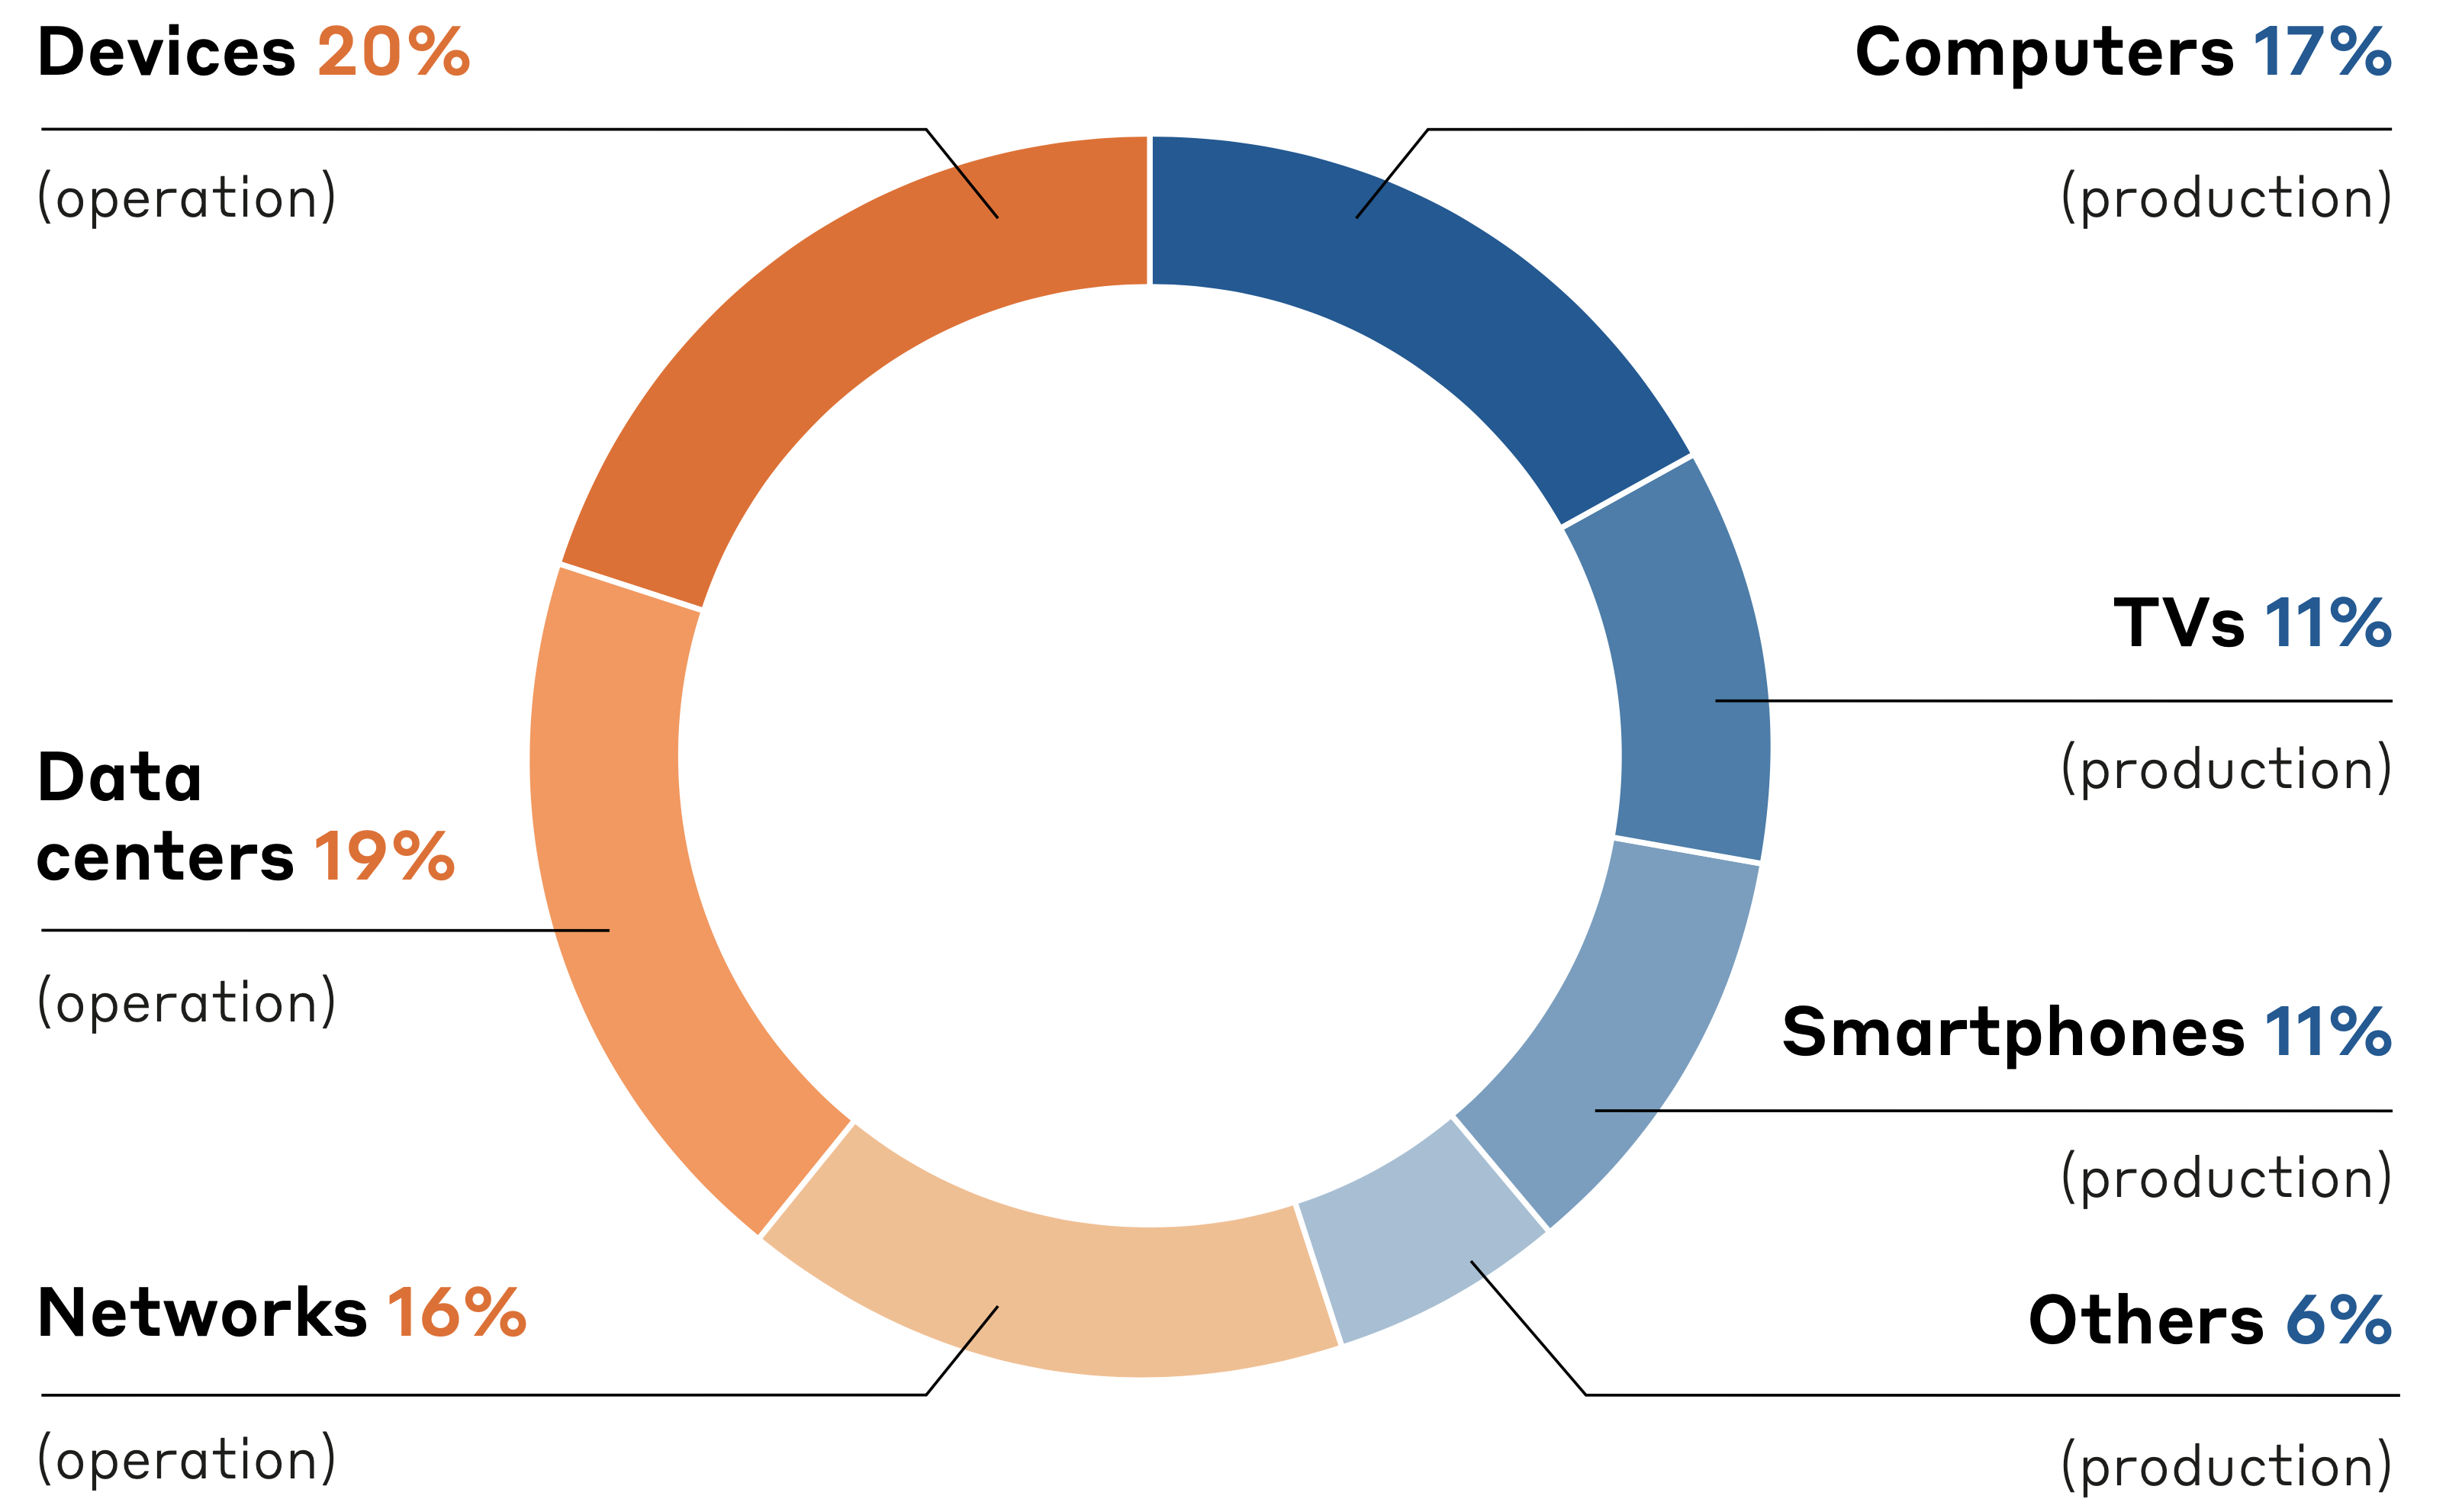
\includegraphics[width=.7\linewidth]{chapters/distribution_of_ict_consumption.png}
    \caption{Final energy consumption of digital technologies by item in 2019(The Shift Project – Forecast Model 2021\cite{shift_2021})}
    \label{fig:distribution_of_ict_consumption}
\end{figure}

Figure~\ref{fig:distribution_of_ict_consumption} shows the distribution of ICT consumption in 2018, where the largest chunk of the energy consumption is due to data usage, aka 63\% of the energy consumed where 22\% of this energy is used by data centers.
Reducing energy consumption means reducing the impact 14\% of the ICT energy consumption has on the environment.

In 2020, the market for data center services was worth 48.9 billion\$.
It is thought that this number will go up to 105.6 billion\$ by 2026~\cite{inshakova2022data}.
This growth is caused mainly by:
\begin{itemize}
    \item shift to remote lifestyle: work, education, and entertainment,
    \item increase in the number of connected devices (IoT),
    \item development of data-hungry technologies such as Machine learning, AI, Big data, and so on,
    \item edge computing and 5G.
\end{itemize}

With this increase in the number of data centers comes an increase in energy consumption, which is a major problem for the environment.
in 2018, data centers consumed around 205 terawatt-hours (TWh)~\cite{schneider2021world}, which is equivalent to the energy consumption of 1\% of the total world's electricity.
This ratio increased up to 1.5 \% in 2020 according to the Journal of Science~\cite{mytton2021data}.
In Figure~\ref{fig:data_centers_power_distribution}, one can see that 40\% of the energy consumed by data centers is used for cooling, while another 40\% is used by the servers themselves.
Therefore, optimizing these two aspects can have a major impact on the energy consumption of data centers.

\begin{figure}[!h]
    \centering
    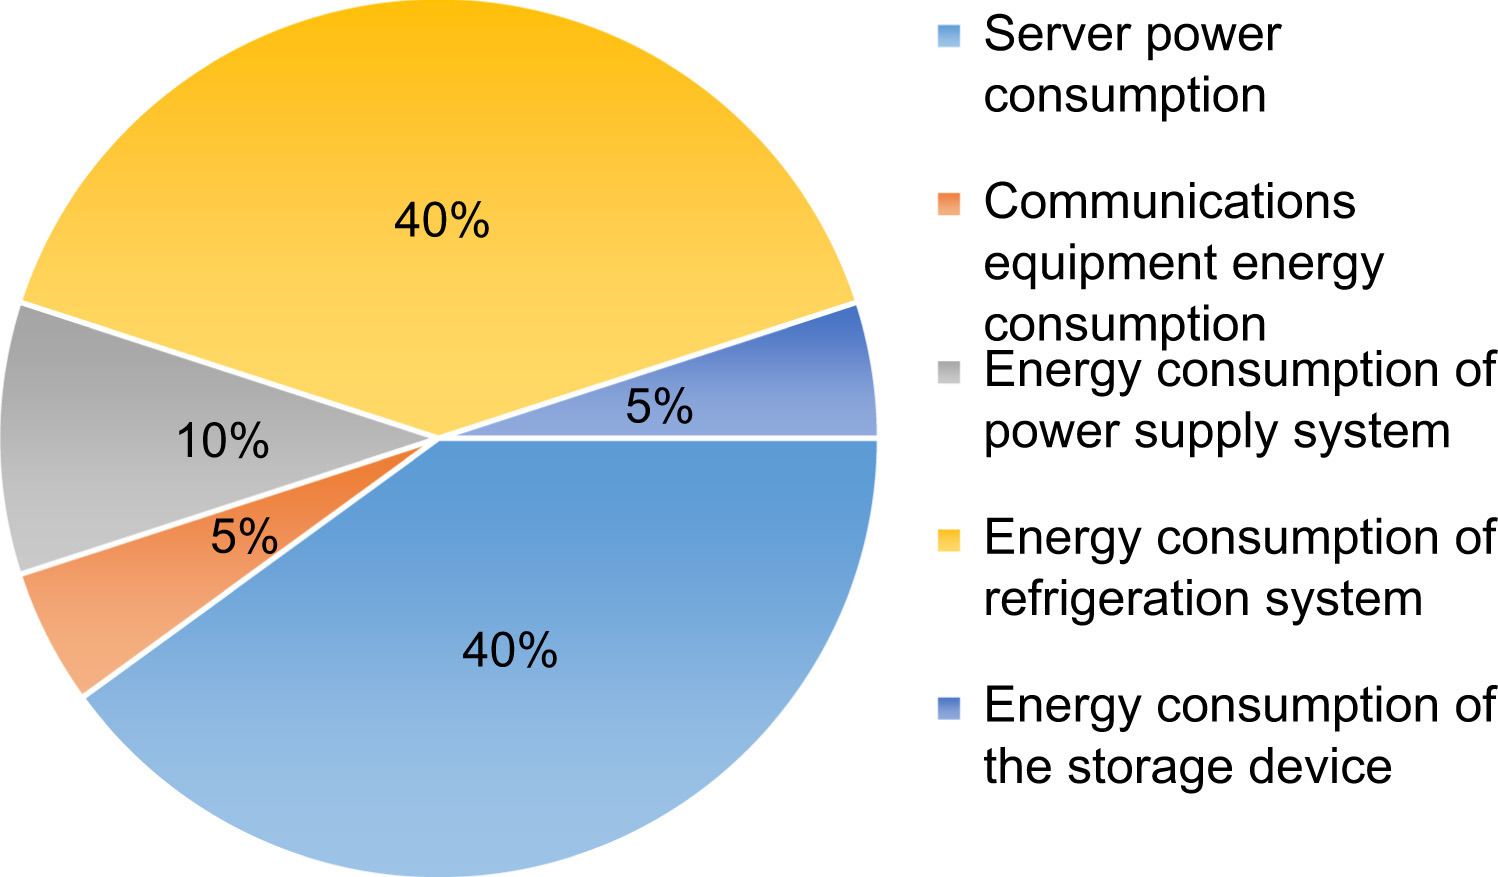
\includegraphics[width=0.6\linewidth]{chapters/data_centers_power_distribution}
    \caption{Distribution of power consumption in a data center~\cite{rong2016optimizing}}
    \label{fig:data_centers_power_distribution}
\end{figure}

Researchers are trying to reduce the energy consumption of data centers through different angles.
Some of the works are focused on the hardware side, such as using new hardware architectures that are more energy-friendly, such as the use of GPUs instead o ARM processors instead of CPUs~\cite{aroca2012towards}.
Others are trying to optimize the cooling system, this can be achieved by using more efficient cooling systems, putting data centers in cold locations or under water~\cite{simon2018project}, or even using the waste heat for other purposes, such as heating buildings~\cite{bouzel2021distributed,cao2021carbon}.

A third approach is to optimize the software, by making software more energy-efficient.
In this thesis, we focus on this approach, and we try to optimize the software by reducing the number of computations that are done by the software.

The best way to do so is to formulate a theory behind the energy consumption of algorithms, such as the complexity and the o notation.
Unfortunately, this is not possible in the current state of the art.
Due to the lack of knowledge about the energy consumption of the algorithms, and the strong correlation between this consumption and the hardware configuration.
Unlike algorithm optimization in the field of performance, which is agnostic toward the platform, the energy consumption of the algorithms is dependent on the execution environment.
Therefore, for the moment, we start by formulating some hypotheses and exploring them using empirical analysis.
Figure~\ref{fig:thesis_position} highlights this thesis's position on the sustainability of ICT\@; while this thesis only addresses a small portion of ICT's energy usage, we feel it is a step in the right direction for additional solutions to mature to preserve humanity.

\begin{figure}[!h]
    \centering
    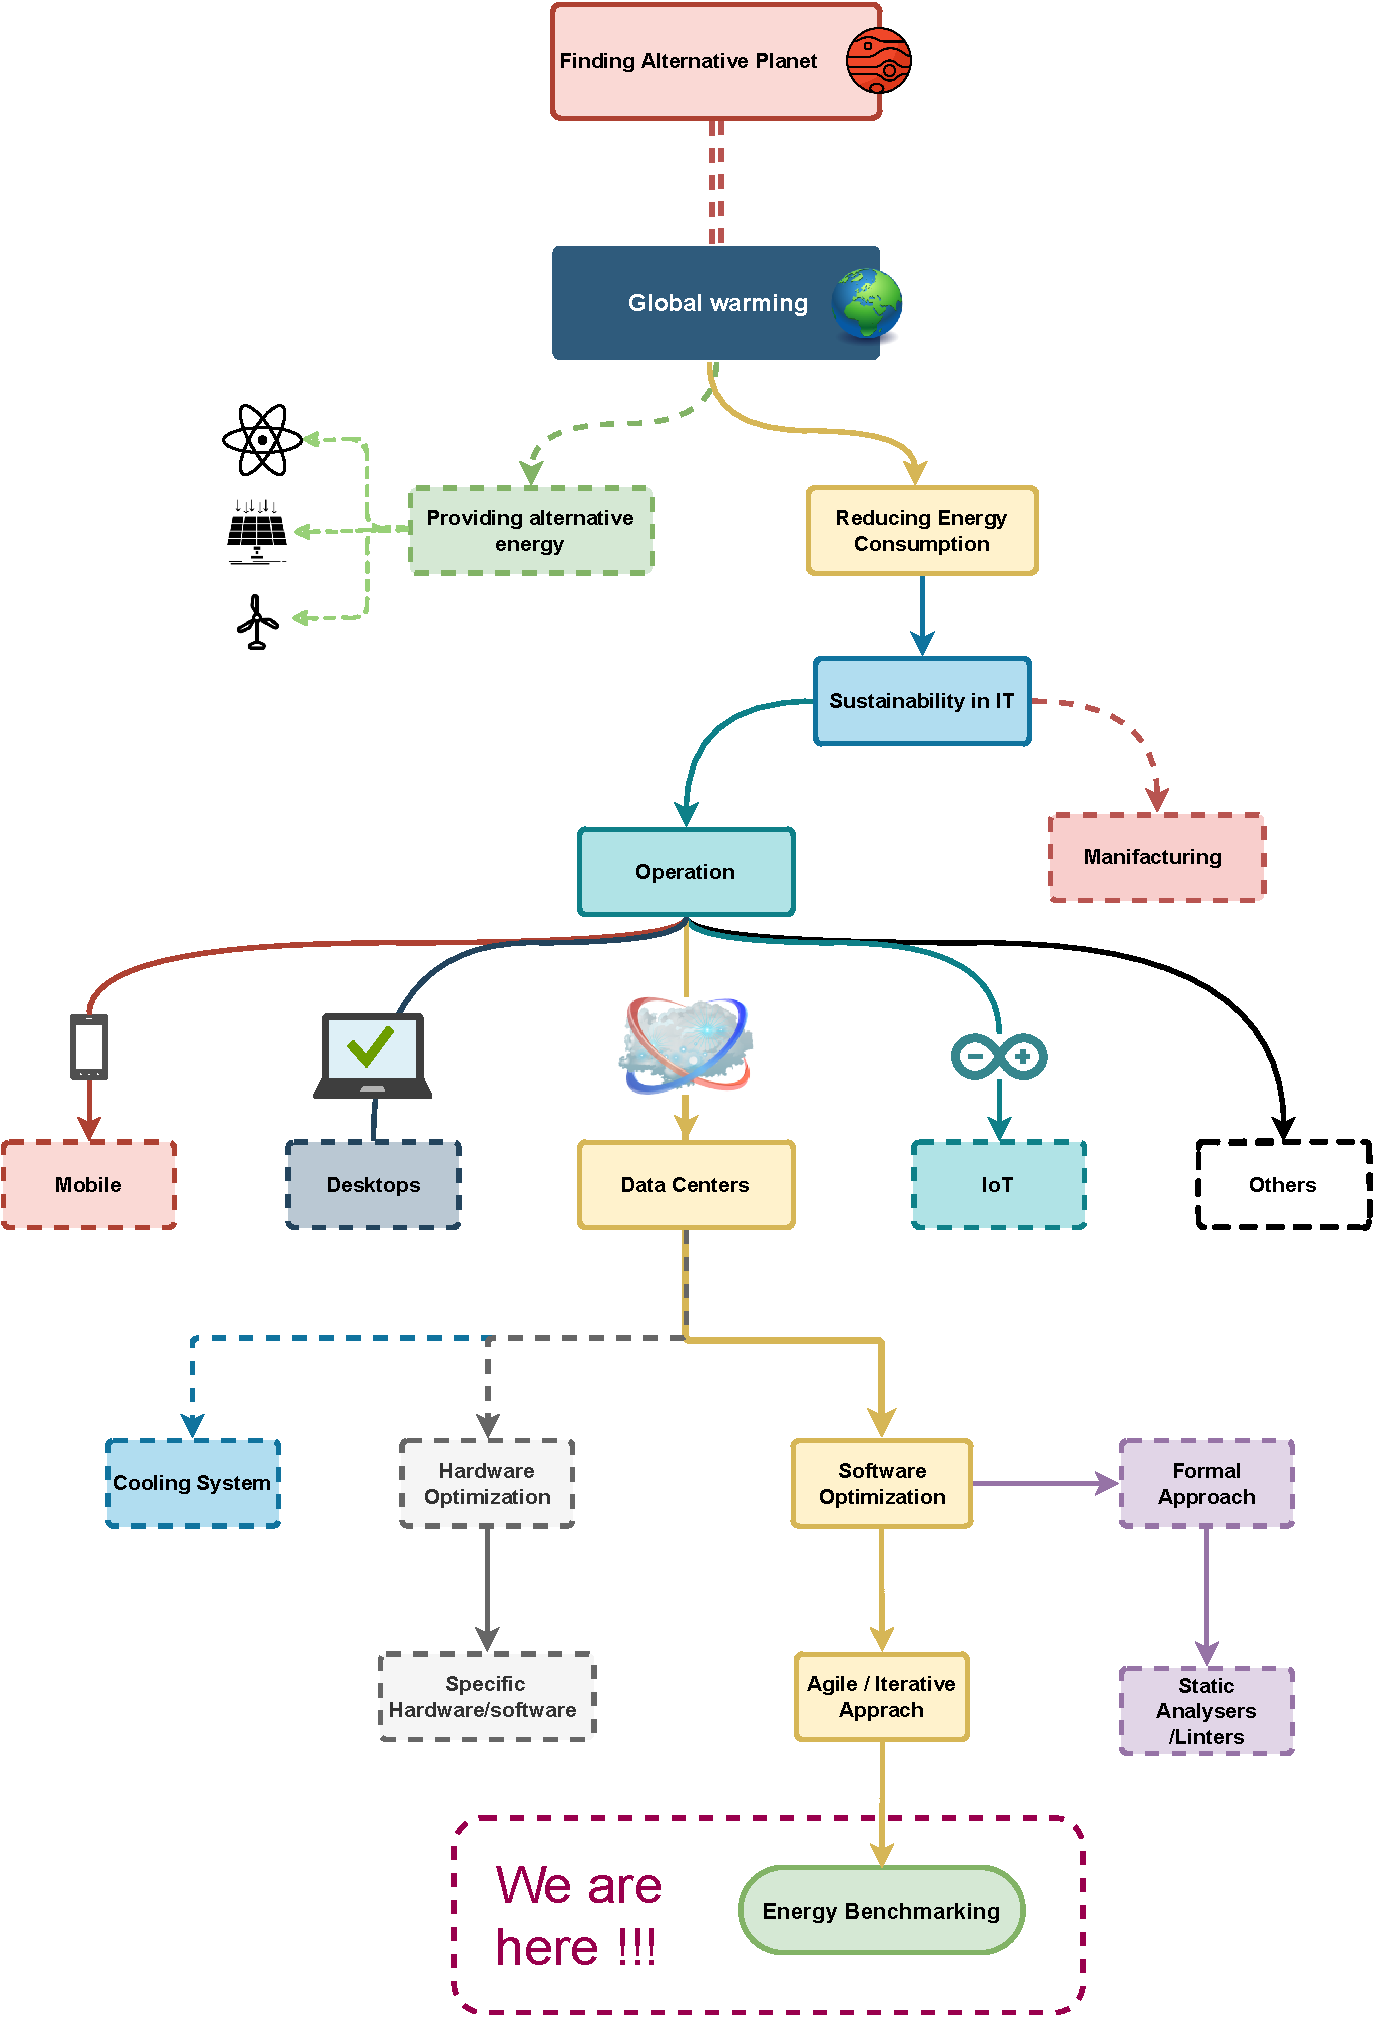
\includegraphics[width=0.7\textwidth,height=\textheight,keepaspectratio]{chapters/thesis_position.pdf}
    \caption{Our position in the IT sustainability research}
    \label{fig:thesis_position}
\end{figure}
\section{Objectives}
The purpose of this thesis is to help developers build more energy-efficient software.
Unfortunately, when it comes to the energy consumption of programs, there is a lack of awareness and knowledge among software developers~\cite{ournani2020reducing,pang2015programmers,pinto2014mining}.
This is mainly due to the lack of tools that can help developers understand the energy consumption of their programs.
Therefore, we aim to provide clear, understandable, and easy-to-use tools and guidelines that can help developers reduce the energy consumption of their programs.

To reduce the energy consumption of software, we can use three strategies.
The first one consists of \emph{reducing energy consumption by reducing the execution time of the program}.
The most intuitive way for developers, as the optimization of software's performance, is a key metric for most programs.
Therefore, in this case, reducing the energy consumption of software becomes a side effect of optimizing the performance of the software.

The second strategy is \emph{optimizing the energy while trying to keep performance}.
In this strategy, we aim to reduce the energy consumption of software without impacting its performance of the software.
This is a more challenging task, as it requires a deeper understanding of the software's energy consumption.
The main focus of this thesis is to provide tools and guidelines that can help developers in this task.

The final strategy consists of \emph{deliberately reducing the performance of the software to reduce its energy consumption}.
The goal of this method is to reduce energy usage by sacrificing execution time.
This strategy is useful while dealing with services since the task has an unlimited execution time.
The second part is to use some. opportunistic schedulers, which will stop the software if it is estimated to spend more energy.
This strategy is discussed first in Chapter~\ref{chapter:porgramming_langauges}, then we continue with this strategy in the perspectives section.

\section{Organization}
\begin{figure}[!h]
    \centering
    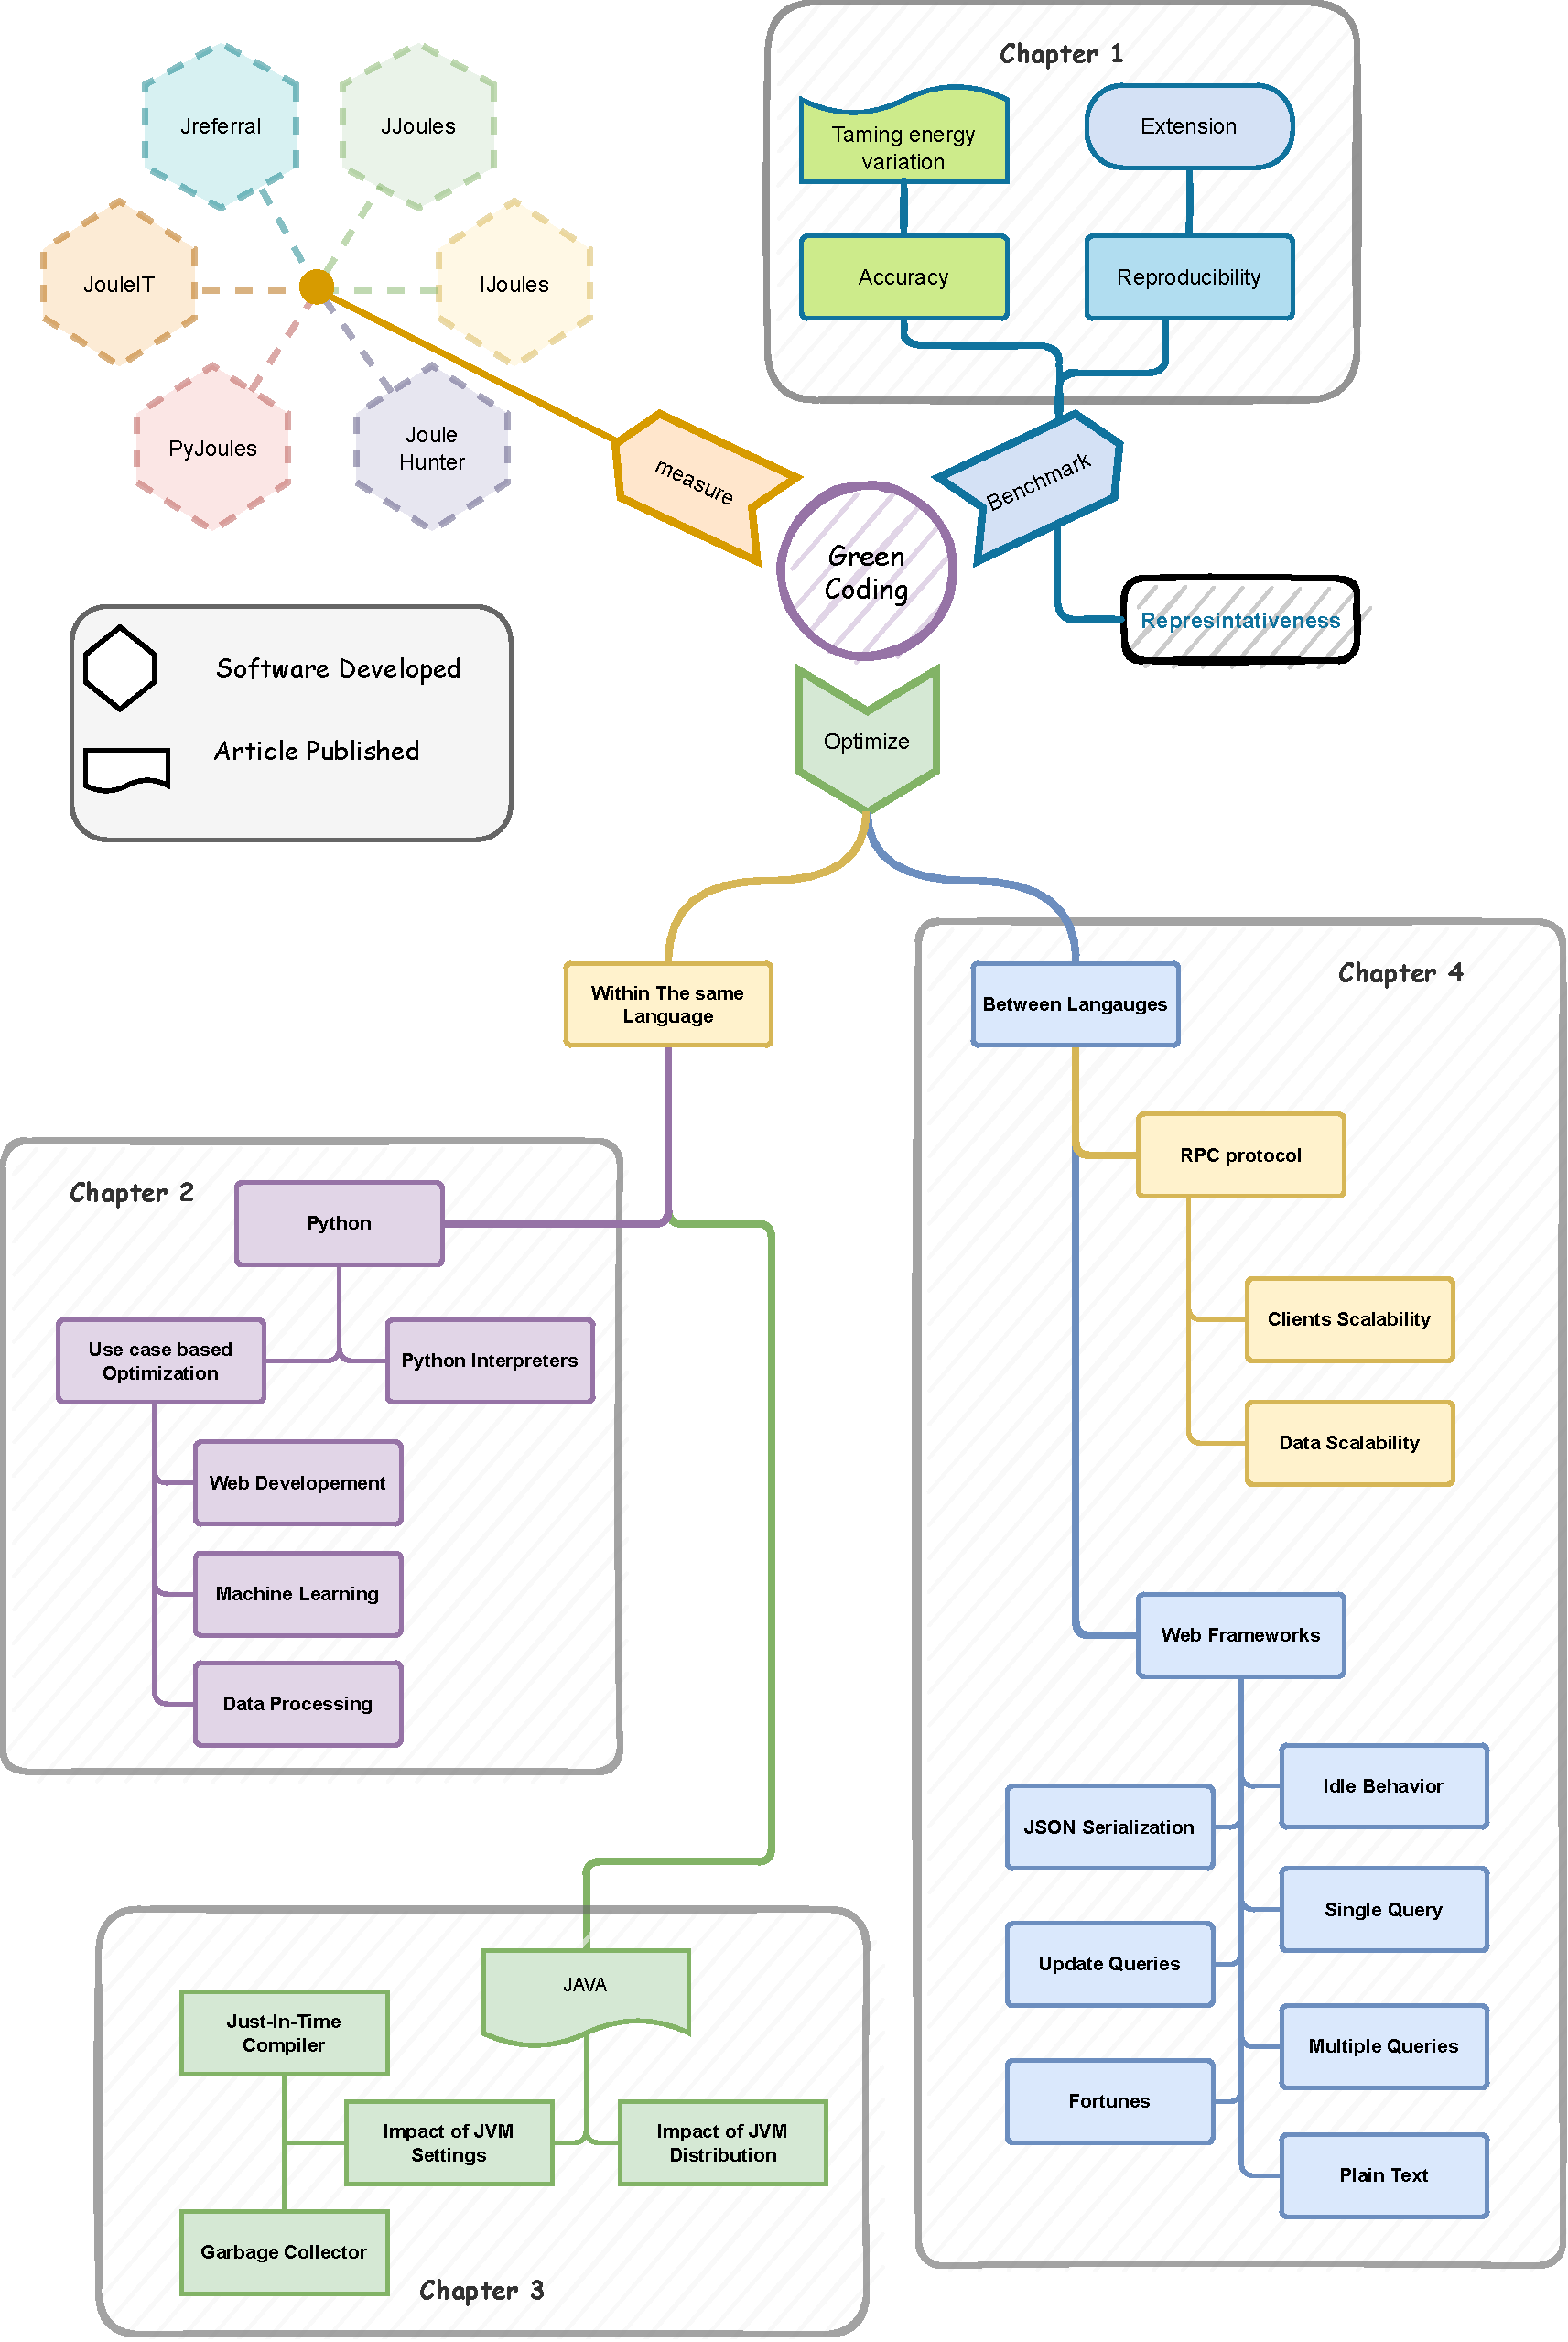
\includegraphics[width=.7\textwidth,height=\textheight,keepaspectratio]{chapters/thesis_contributions.pdf}
    \caption{Contributions reported in this thesis}
    \label{fig:thesis_contributions}
\end{figure}

Figure~\ref{fig:thesis_contributions} summarizes the work completed for this thesis As mentioned in the previous section, our goal is to help developers reduce the energy consumption of their programs during execution.
We use an empirical approach to accomplish this.
As a result, we require some tools to assist us in this task.
To begin, we provide a tool to assist developers in measuring the energy consumption of their programs.
The rest of the manuscript is outlined below.

\begin{itemize}
    \item Chapter~\ref{chapter:literature_review} provides a literature review of the energy consumption of software.
          First, it introduces the challenges that one can encounter when running an empirical study, \emph{reproducibility}, \emph{accuracy}, and \emph{representativeness}, the ways in the state of the art overcome these challenges in the field of computer sciences.
          Then, it narrows down to the energy consumption of software and the challenges that one can encounter when measuring the energy consumption of software.
          In this section, we provide the literature approaches used to measure energy consumption and classify them, compare them and discuss their pros and cons when used for our research. After that, we tackle the challenge of accuracy within the field of energy consumption and discuss how the literature tried to overcome these challenges. Finally, we  present some of the most recent works in the field of software energy consumption optimization;
          % We conclude this chapter by providing a simple method that we will use for the rest of the thesis to optimize the energy consumption of software. \textbf{BMO} : benchmark , measure and optimize.  
    \item Chapter~\ref{chapter:benchmarking} discusses two facets of empirical tests and how we adapt them to energy consumption measurements.
          First, we discuss the reproducibility challenge and how to overcome it with the usage of containers, then we push this approach further by proposing and new protocol to make tests not only reproducible but able to be extended with other features to overcome the rapid pace of software evolution.
          The second part of this chapter discusses the aspect of accuracy when it comes to energy consumption measurements.
          This section demonstrates how energy measurements might differ and produce conflicting results for the same work when run on identical machines or even the same machine.
          Then, it provides some solutions to reduce this energy variation and improve the accuracy of the measurements;
    \item After setting the ground for energy benchmarks in the previous chapter, we discuss the energy consumption of Python, one of the world's most popular programming languages.
          Chapter~\ref{chapter:python} reports on how much python costs in terms of energy consumption compared to other languages.
          Then, it provides some statistics about its popularity and typical use cases and studies the impact of Python on energy consumption in three typical use cases, machine learning, web servers, and data manipulation.
          For each use case, we compare the energy consumption of several approaches and provide guidelines on how to optimize the energy consumption of python programs in these use cases.
          Finally, we provide a non-intrusive way to optimize energy consumption without altering the code of the program.
          We achieve this by using a different implementation of the Python interpreter.
          This not only allows developers to spend less time optimizing their code but also allows them to use it on the legacy code that they cannot modify;
    \item Motivated by the outcomes of the non-intrusive optimization, we follow this strategy on one of the most popular legacy code base applications programming languages, Java.
          In Chapter~\ref{chapter:java}, we try to optimize the Java code, using by changing the default JVM implementation.
          We compare the energy consumption of $12$ benchmarks using $52$ implementation, each benchmark is dedicated to a typical use case.
          After that, we study two of the JVM features, JIT and GC, and show their impact on the energy consumption of the Java code;
    \item In contrast, Chapter~\ref{chapter:porgramming_langauges}  uses the flexibility provided by the micro-services architecture~\cite{dmitry2014micro} to analyze each programming language's energy behavior in light of various web scenarios to optimize the energy use of web services.
          We first examine the effects of the various programming languages when dealing with the \emph{Remote Procedure Call} (RPC) Protocol.
          In this instance, we use two scaling factors: the number of concurrent clients and the size of the requests. Then, we compare $261$ web frameworks, each implementing the same website using seven use cases.
          This analysis aims to look at how each technology uses energy in different kinds of web situations.
    \item Finally, we conclude our work in Chapter~\ref{chapter:conclusion} by summarizing the work done in this thesis and discussing the future work that can be done to further reduce the energy consumption of software.
\end{itemize}

% First, we create a benchmarking protocol that serves researchers and practitioners, experimenting with their approaches and solutions to reduce the energy consumption of programs.
% Then, using this protocol, we analyze and try to optimize the energy consumption of one of the most popular programming languages, Python. We first study python within its most use cases, machine learning, and web Development. Then we try to optimize the energy consumption on the outer side, this can be achieved by targeting the interpreter itself.
% After that, we continue our non-intrusive approach, by targeting the impact of the virtual machine on the JAVA code. This not only helps practitioners improve their software energy without changing their code, but is also beneficial for reducing the energy consumption of the legacy code with almost zero cost.
% Finally, we will shift our focus to other programming languages and compare the energy consumption of different programming languages.
% We consider two main use cases. The RPC protocol, and web servers.

% we have three scenarios, to reduce energy consumption :
% 1. win-win, reducing energy consumption by enhancing the performance: the first one is done by default by most of the developers and performance engineers, which is to optimize the code itself
% 3. win neutral, reducing energy consumption while keeping the same performance: the second one is finding reducing the energy consumption while trying to keep the same performance, which the work of this theses 
% 2. win loose, reducing energy consumption by reducing the performance: optimizing  the energy consumption by sacrificing the performance of the program itself which is what we call  green faas  we will talk about this in the perspective section


% \url{https://www.statista.com/statistics/871513/worldwide-data-created/}
% https://www.iea.org/reports/data-centres-and-data-transmission-networks

% Our work will be presented in the following chapters:
% \begin{enumerate}
%     \item \ref{chapter:literature_review}: Where we discuss the work done on energy consumption and optimization in software engineering
%     \item \ref{chapter: benchmarking}: It will present a set of guidelines and tools to help practitioners measure the energy consumption of their algorithms.
%     \item: it will discuss the behavior of python and the possible ways to tune it in order to reduce the energy consumption
%     \item: will present a study on java programming language and the impact of the JVM choice on the energy consumption
%     \item: we will present the impact of programming languages on the energy consumption of the algorithms especially when it comes to web services.
%     \item: as a perspective, we introduce the impact of parallelism on energy consumption in time-agnostic cases
% \end{enumerate}
% \subsection*{Contributions}


\section{Contributions}
The contributions of this thesis are summarized as follows:
\subsection*{Conferences}
\nobibliography*
\begin{enumerate}
    \item \bibentry{ournani2020taming},
    \item \bibentry{ournani2021evaluating}.
\end{enumerate}

\subsection*{Tools}
% \begin{itemize}
%     \item \textbf{Jouleit} (\url{github.com/powerapi-ng/jouleit}):  \bibentry{Belgaid_JouleHunter_an_2021},
%     \item \bibentry{Belgaid_JRefferal_Which_JVM_2021},
%     \item \bibentry{Belgaid_Jouleit_a_2020},
%           % \item \bibentry{Belgaid_Ijoules_Python_library_2020}
%     \item \bibentry{Belgaid_Pyjoules_Python_library_2019}.
% \end{itemize}
\begin{itemize}
    \item \textbf{Jouleit} (\url{github.com/powerapi-ng/jouleit}): a tool that can be used to monitor energy consumption for any Linux program, this tool was used to compare the energy consumption of different JVMs;
          \\
          \bibentry{Belgaid_Jouleit_a_2020},
    \item \textbf{JRefferal} (\url{github.com/chakib-belgaid/jreferral}): a tool that allows the user to explore the JVM settings and their impact on the energy consumption of a given Java program. This tool was the result of the second article of this thesis;
          \\
          \bibentry{Belgaid_JRefferal_Which_JVM_2021},
    \item \textbf{PyJoules} (\url{pypi.org/project/pyJoules}) is a software toolkit to measure the energy footprint of a host machine along the execution of a piece of Python code. It can measure the energy consumption on the level of script, function, and bloc of code;
          \\
          \bibentry{Belgaid_Pyjoules_Python_library_2019},
    \item \textbf{JouleHunter} (\url{pypi.org/project/joulehunter}): an energy profiler for python applications. It can be used to highlight the functions that consume the most energy in a given Python program. Its main usage is to help developers do an exploratory analysis of their application to scope the functions that should be optimized to be then targeted by PyJoules;
          \\
          \bibentry{Belgaid_JouleHunter_an_2021},
    \item \textbf{GreenBoard} (\url{github.com/chakib-belgaid/greenboard}): a dashboard designed to help developers choose the best stack for their web application. It is based on the results of the third article of the last chapter.
\end{itemize}

% \subsection*{Future Work}
% \begin{itemize}
%     \item Reducing the energy consumption of Python using non-intrusive techniques,
%     \item Empirical analysis on the energy consumption of different web frameworks,
%     \item The impact of programming languages on energy consumption of web services (a case study of RPC protocol),
%     \item How do ORMs affect how much energy is used? A case study of Django and Flask.
% \end{itemize}

% \cleardoublepage

\newpage
\chapter{Problem Background}
\label{chapter:problem_background}


\cleardoublepage

\chapter{State of the Art}
\label{chapter:literature_review}
\import{chapters/literature/}{draft_citations}

\newpage

\chapter{Empirical Evaluation Protocol}
\label{chapter:testing}

In order to optimize the energy consumption of software we first want to setup a experemental enviroment. We have chose to use the empirical appraoch so we will reduce the energy consumption with trial and error.

%  This chapter will be dedicated to provide a set of guidelines to provide a \em{reproducible, accurate} and \em{representative} tests. Each aspect will be detailed in the sections below. 

\import{chapters/testing/}{challenges}
\import{chapters/testing}{stateoftheart}
\import{chapters/testing/}{environement}
\import{chapters/testing/}{experement}
\import{chapters/testing/}{conclusion}


\chapter{Energy Footprint of Programming Languages}
\label{chapter:porgramming_langauges}
In this chapter, we study how the programming language affects the energy the software consumes.
We suggest starting with general micro-benchmarking and watching how each programming language performs with the CPU and memory.
The main goal of this chapter is to advise developers on how to choose a programming language based on their project's needs in order to make their product use the least amount of energy possible.
For such a question, no answer is obvious.
Nonetheless, there are some features we can take from each programming language, such as: 
\begin{itemize}
    \item performance,
    \item community support,
    \item scalability,
    \item energy consumption,
    \item memory usage.
\end{itemize}

As we saw in the last chapter, one of the most important things about a test is how well it \textsc{represents} the production environment.
Therefore, we extend this study to include real-world use cases, with two case studies provided in the parts that follow. 

\section{Investigating Remote Procedure Call Frameworks}
\import{\currfiledir/rpc}{rpc}

\section{Investigating Web Application Frameworks}
\import{\currfiledir/web_frameworks}{web_frameworks}
\newpage

\chapter{Execution enviroment}
\label{chapter:enviroment}
After studying the impact of the programming languages choice on the energy consumption of softwares. we wanted to dig in more deeper. Therefore we have chosen two of the most popular programming lanaguages \textbf{Python} and \textbf{Java}
In this chapter we will reduce the energy consumption of those following lanaguages by doing some tuning
\import{chapters/execution_environement/java}{java}

\clearpage
\chapter{Discussion and Conclusion}
\label{chapter:conclusion}

This manuscript reports on several contributions to measuring and reducing software energy consumption.
We used a three-step strategy to lower software energy: benchmarking, measuring, and optimizing.
We started with the benchmarking phase.
Chapter~\ref{chapter:literature_review} discussed the challenges of a successful benchmarking strategy: reproducibility, accuracy, and representativeness.
We concluded that software containers, like "Docker", would be the best fit to ensure that energy studies could be reproduced.
We then extended this reproducibility to an evolving protocol that helps researchers keep up with the rapid pace of software development.
Then, we targeted the accuracy by studying the hardware and software factors that can impact the energy variation and how practitioners can tune them to harness this energy variation.

After establishing a robust benchmarking protocol to create energy-based experiments, we shifted our focus to the optimization side.
We opted to start with Python, the most popular yet energy-hungry programming language.
As a result, we began by examining the energy behavior of Python code in its most common usage.
Then, we presented a non-intrusive method to lessen its energy use.
Following that, we applied the same strategy to another programming language known for its legacy code base, Java, to prove that we can still cut the energy usage of existing running applications without incurring high costs.

Lastly, we used the flexibility of the micro-services architecture to look at how each programming language uses energy in different web scenarios.
We first examined the effects of the various programming languages when dealing with the \emph{Remote Procedure Call} (RPC) protocol.
Then, we extended this study to a more practical application by comparing $261$ web frameworks, each implementing the same website using seven use cases.
Then, we provided practitioners with a dashboard to determine which stack is best for a given situation.


\section{Summary of Contributions}
\label{section:SummaryofContributions}
The contributions reported in this thesis are covered in this section.
The following is a summary of them:

\subsection{Published Papers}
This part summarizes the contributions that have been already accepted in conferences and journals.

\begin{enumerate}
      \item \textbf{Taming energy consumption variations in systems benchmarking}:
            We investigate the phenomenon of variation when measuring the energy consumption of experiments in this study.
            In this paper, we discuss various hardware and software factors that can amplify variations in recorded energy measures, with a focus on the following research questions:
            \begin{description}
                  \item[\textsc{RQ}~1:] Does the benchmarking protocol affect the energy variation?
                  \item[\textsc{RQ}~2:] How important is the impact of the processor features on the energy variation?
                  \item[\textsc{RQ}~3:] What effect does the operating system have on energy variation?
                  \item[\textsc{RQ}~4:] Does the choice of processor make a difference in reducing the energy variation?
            \end{description}

            This contribution shows how processor features can significantly affect the variation in energy use between the benchmarking protocol and the operating system.
            Finally, this study presents several guidelines for controllable parameters that practitioners could easily change to increase the accuracy of their experiments.

            \bibentry{ournani2020taming}


      \item \textbf{Evaluating the impact of Java virtual machines on energy consumption}:
            In this paper, we thoroughly investigate how JVMs affect software energy usage.
            To address the following research concerns, we reveal through this study several trials on hundreds of JVMs versions provided by various providers:
            \begin{description}
                  \item[\textsc{RQ}~1:] What is the impact of existing JVM distributions on the energy consumption of Java-based software services?
                  \item [\textsc{RQ}~1:] What are the relevant JVM settings that can reduce the energy consumption of a given software service?
            \end{description}
            The findings demonstrate that choosing the right JVM platform can significantly reduce energy usage depending on the software and use case.
            This optimization can also be achieved by properly configuring the JIT and GC parameters.

            \bibentry{ournani2021evaluating}
\end{enumerate}

\subsection{Softwares and Tools}
While the benchmarking and optimization parts were presented as chapters in this thesis, the measurement part was primarily based on developing tools that measure the energy consumption for a given use case.
The following is a summary of the tools that were developed during this thesis:
\begin{itemize}
      \item \textbf{Jouleit} (\url{github.com/powerapi-ng/jouleit}): a tool that can be used to monitor energy consumption for any Linux program, this tool was used to compare the energy consumption of different JVMs;
      \item \textbf{JRefferal} (\url{github.com/chakib-belgaid/jreferral}): a tool that allows the user to explore the JVM settings and their impact on the energy consumption of a given Java program. This tool was the result of the second article of this thesis;
      \item \textbf{PyJoules} (\url{pypi.org/project/pyJoules}) is a software toolkit to measure the energy footprint of a host machine along the execution of a piece of Python code. It can measure the energy consumption on the level of script, function, and bloc of code;
      \item \textbf{JouleHunter} (\url{pypi.org/project/joulehunter}): an energy profiler for python applications. It can be used to highlight the functions that consume the most energy in a given Python program. Its main usage is to help developers do an exploratory analysis of their application to scope the functions that should be optimized to be then targeted by PyJoules;
      \item \textbf{GreenBoard} (\url{github.com/chakib-belgaid/greenboard}): a dashboard designed to help developers choose the best stack for their web application. It is based on the results of the third article of the last chapter.
\end{itemize}



\subsection{Future Submissions}
\begin{itemize}
      \item Reducing the energy consumption of Python using non-intrusive techniques,
      \item Empirical analysis on the energy consumption of different web frameworks,
      \item The impact of programming languages on energy consumption of web services (a case study of RPC protocol),
      \item How do ORMs affect how much energy is used? A case study of Django .
\end{itemize}

\section{Future Work\note{ In Draft }}
While our contributions are a good start to the energy-aware software engineering field, there are still many challenges to overcome. This is just the tip of the iceberg. The following are some of the challenges that we would like to address in the future:

\subsection{Short Term Challenges}
Before starting a journey looking for a new mine, one should first look at the resources available to him. In the same way, we need to first look at the resources available to us before we start looking for new challenges. The following are some of the challenges that we can address in the short term:

\paragraph{The evolution of python interpreters}
In Chapter \ref{chapter:python} we compared several python interpeters. However, most of these alternative solutions were based on python2 which is now deprecated. On the other hand, the default python interpreter (aka . CPython) has included many features and optimization since our last study, such as the introduction of Python introduced the \texttt{dataclasses} in version 3.7 (PEP 557\footnote{\url{https://peps.python.org/pep-0557/}}) that can be used to reduce the memory footprint of python objects,
the new parser in python 3.9~\footnote{\url{https://docs.python.org/3/whatsnew/3.9.html}}, the user type alias in python3.10~\footnote{\url{https://peps.python.org/pep-0613/}}.
And the most interesting changes for us occurred in CPython 3.11 which is claimed to be 25\% faster than python 3.10 \footnote{\url{https://github.com/faster-cpython/ideas}}. We need to re-evaluate the impact of these changes on the energy consumption of python programs.

\paragraph{The impact of ORMS}
We continue with our work with Python, and this time we will delve deeper into the impact of the ORMS, As shown in Section\ref{sec:webdev}, The ORMs are the most energy-consuming part of a web application. We intend to widen this analysis to other python ORMS such as SQLAlchemy\link{https://www.sqlalchemy.org/} and Peewee\link{http://docs.peewee-orm.com/en/latest/}. We will also explore the real relationship between the ORM, the database, and the web framework.

\paragraph{Python and machine learning}
In chapter \ref{chapter:python}, we showed that training accuracy has a huge cost on the energy using a single model. However, in the real world, we often use multiple models to solve a problem. We will explore the impact of using multiple models on the energy consumption of a machine learning application As well as compare the energy consumption of different machine learning frameworks such as PyTorch\link{https://pytorch.org/}, scikit-learn\link{https://scikit-learn.org/stable/} and TensorFlow \link{https://www.tensorflow.org/}.



\paragraph{ Which is the greenest couple? a comparative study of JVMs and JVM-based programming languages}
As we have seen in Chapter \ref{chapter:java} the choice of the JVM can greatly impact the energy consumption of the program. On the other hand, we have seen in Chapter \ref{chapter:porgramming_langauges} that other JVM-based languages depicted half power consumption of the JAVA code, was it only because of the web framework ? or there is a real difference between the JVMs and the JVM based languages? We will explore this question by comparing the energy consumption of different JVMs and JVM-based languages such as Scala, Kotlin, Groovy, and Clojure.

\paragraph{the impact of programming languages on energy consumption, do translators helps in reducing the energy cost of a program?}
One of the hardest challenges when comparing the energy consumption of multiple programming languages was the bias of the expertise of the programmer. One solution was to create a reference benchmark that allows one to compare several programming languages \link{https://benchmarksgame-team.pages.debian.net/benchmarksgame/index.html}, this was used for many researchers such as the work of \citeauthor{couto2017towards} \cite{couto2017towards}, others were to use some basic algorithms like \cite{noureddine_preliminary_2012} where they compare the energy consumption using the Hanoi tower problem \link{https://en.wikipedia.org/wiki/Tower_of_Hanoi} using different programming languages using the same algorithm.or other simple benchmarks using the Rosettacode base \link{https://rosettacode.org/wiki/Rosetta_Code}
however, this scope is limited to single algorithms. and does not help cover the production mode, this is why we shifted to the web frameworks.  Now that our semanticc analyzers issued from the OpenAI project\link{https://openai.com/} like the automatic test generator ponicode\link{https://www.ponicode.com/} and the ai code generator \link{https://github.com/features/copilot}
an interesting new feature provided by the GitHub copilot is GitHub copilot labs\link{https://githubnext.com/projects/copilot-labs/} is the ability to automatically translate the code from one language to another. We will explore the impact of this feature on the energy consumption of a program.


\paragraph{raising awareness of the energy consumption of the Softwares}
While this thesis's main focus was to optimize energy consumption using comparative studies, it was easier to say that approach X is greener than approach Y no matter which metric we were using. however, it won't be the case for developers while measuring the energy consumption of their programs, some tried to give labels such as (A,B,C ..etc) while others translated these raw metrics in an equivalent of fuel consumption (e.g. 1 liter of fuel per 1000 lines of code). most of the approaches were to use the carbon emission, such as\cite{patterson2021carbon} or ecograder~\link{https://ecograder.com/}
we will explore these approaches and see how they can be used to rise awareness of the energy consumption of their code



\subsection*{Representativeness}:

As we have seen in the state of the art, a successful benchmark meets three criteria, reproducibility, accuracy, and representativeness, During this thesis we discussed two of these criteria, reproducibility, and accuracy, however, we did not discuss the representativeness of our benchmarks. We relied on state-of-the-art benchmarks to represent real-world applications. However, the gap between these benchmarks and the industry is getting bigger and bigger due to the extreme pace of the software development. In this Section, we will tackle the issue of representativeness and discuss how we can improve our protocol to fit real-world applications.
What is the purpose of doing optimizations if they cannot be applied to real-world applications?

First, we will consider taking advantage of the popularity of CI/CD among developers to provide some insights into the energy consumption of their code.
We did provide a sonar tool with our intern that can provide the energy consumption of JAVA-based code repository, figure~\ref{fig:JunitSonarplugin} shows the work of our intern that used a sonar plugin to highlight the energy evolution of java application across the time. This prototype got even more sophisticated to become Joule-dff\link{https://github.com/davidson-consulting/diff-jjoules}  is a tool to be added in the project continuous integration in order to highlight the energy evolution of the java programs.
We intend to push this even further to detect the  commits responsible for an increase or the optimization within the source code

\begin{figure}[!h]
      \centering
      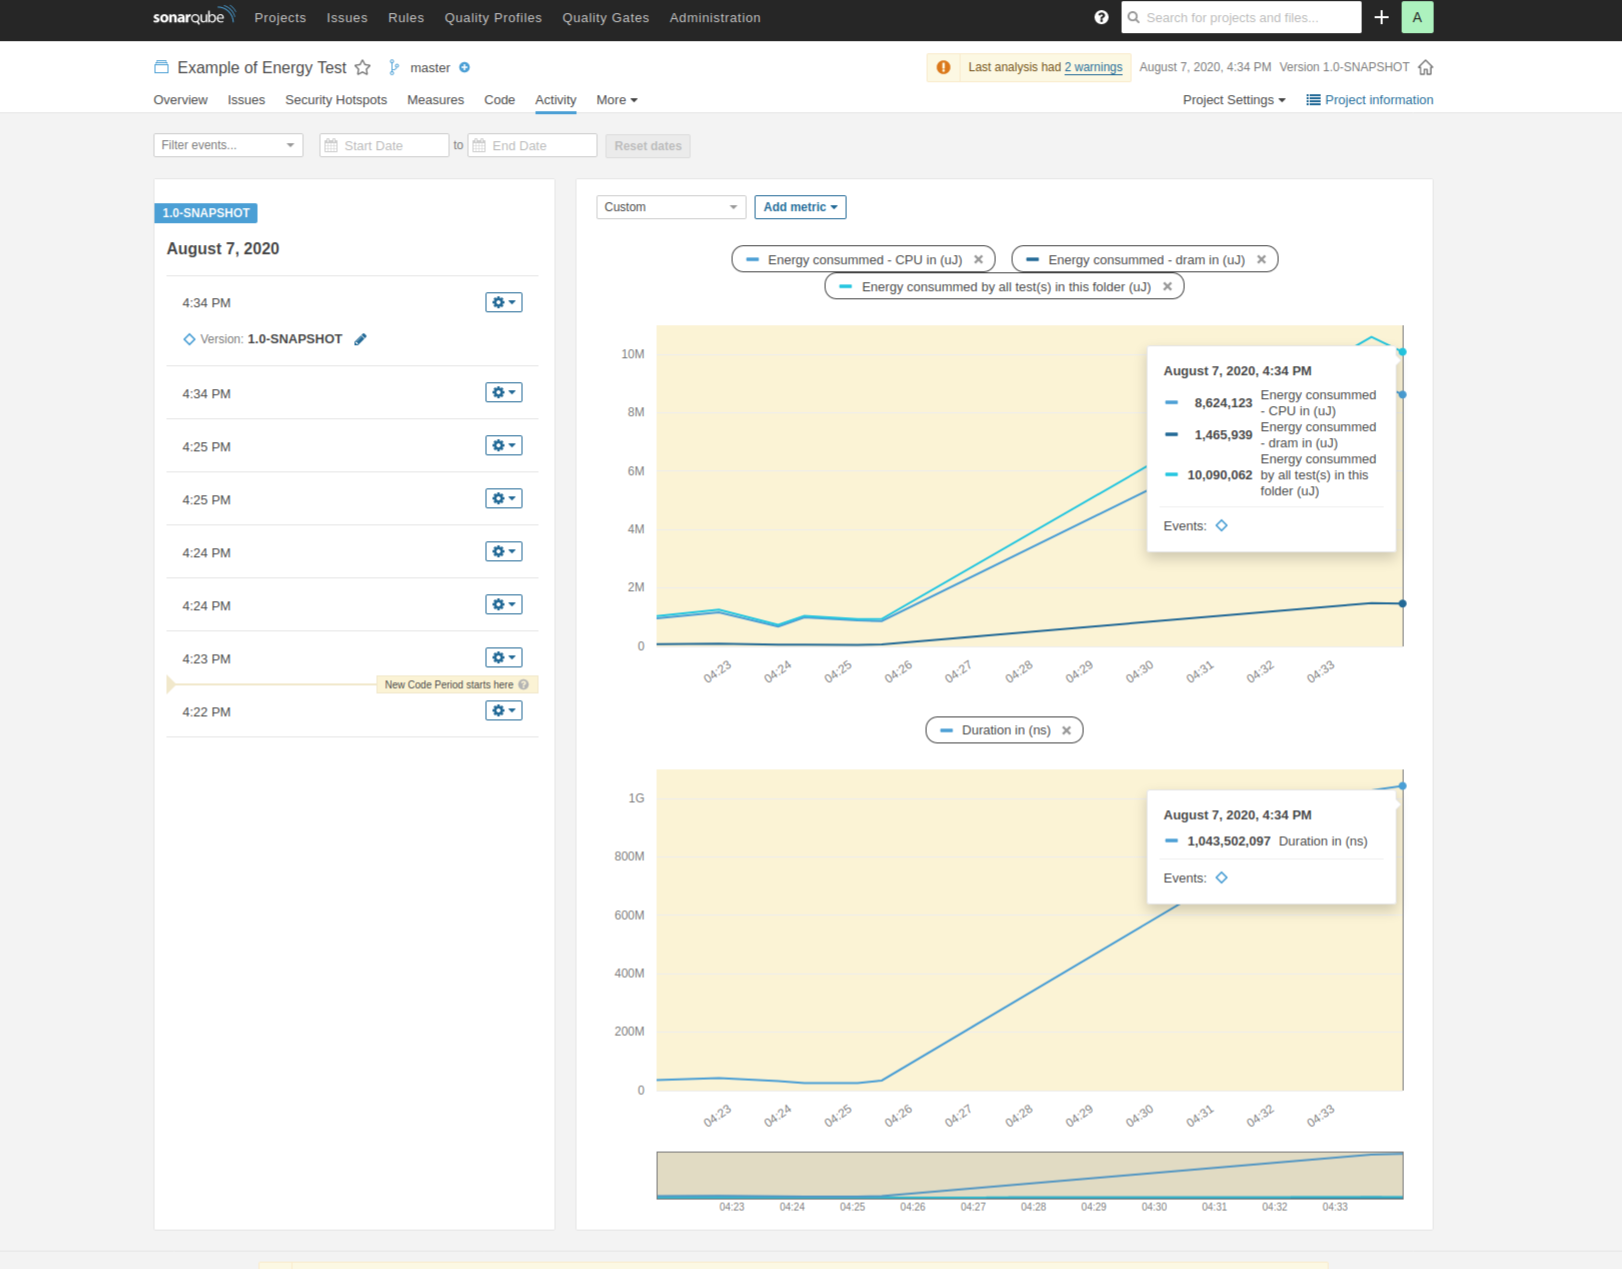
\includegraphics[width=0.8\linewidth]{chapters/JunitSonarplugin}
      \caption{Sonar plugin for Junit}
      \label{fig:JunitSonarplugin}
\end{figure}

we urge energy-efficiency benchmark developers to report measurements at nonpeak activity levels for a more complete characterization of a system's energy behavior\cite{barroso2007case}.


\subsubsection*{greenFaas}
servers operate most of the time at between 10 and 50 percent of their maximum utilization levels \cite{barroso2007case}


\begin{enumerate}

      \item lazy code, sacrificing the performance in order to get a better energy consumption --> green faas
      \item more representative benchmarks, using several CPU saturation levels
      \item measuring the energy impact instead of the row energy consumption. ( the highway analogy when a single application consumes less energy, however the total energy consumption of the system increases )
\end{enumerate}
\vfill \strut  % to fill the rest of the page with blank lines
\cleardoublepage
\begin{appendices}
\newpage
\addcontentsline{toc}{chapter}{APPENDICES}   

\chapter{Full Results:....}
\label{chapter:appendix_experimental_results_1}
\setcounter{table}{0}
\renewcommand{\thetable}{A.\arabic{table}}
\setcounter{figure}{0}
\renewcommand{\thefigure}{A.\arabic{figure}}

\newpage
\section*{Sequence 0}






\chapter{Full Results: ...}
\label{chapter:appendix_experimental_results_2}
\setcounter{table}{0}
\renewcommand{\thetable}{B.\arabic{table}}
\setcounter{figure}{0}
\renewcommand{\thefigure}{B.\arabic{figure}}
 
 
 
\newpage 
\section*{Sequence 0} 


 

\end{appendices} % Appendices

% ********************************** Back Matter *******************************
% Backmatter should be commented out, if you are using appendices after References
%\backmatter

% ********************************** Bibliography ******************************
\begin{spacing}{0.9}

    % To use the conventional natbib style referencing
    % Bibliography style previews: http://nodonn.tipido.net/bibstyle.php
    % Reference styles: http://sites.stat.psu.edu/~surajit/present/bib.htm

    \bibliographystyle{apalike}
    %\bibliographystyle{unsrt} % Use for unsorted references  
    %\bibliographystyle{plainnat} % use this to have URLs listed in References
    \cleardoublepage
    \bibliography{static_final_library} % Path to your References.bib file


    % If you would like to use BibLaTeX for your references, pass `custombib' as
    % an option in the document class. The location of 'reference.bib' should be
    % specified in the preamble.tex file in the custombib section.
    % Comment out the lines related to natbib above and uncomment the following line.

    %\printbibliography[heading=bibintoc, title={References}]


\end{spacing}

% ********************************** Appendices ********************************

% \begin{appendices} % Using appendices environment for more functunality

%     \include{Appendix1/appendix1}
%     \include{Appendix2/appendix2}

% \end{appendices}

% *************************************** Index ********************************
\printthesisindex % If index is present

\end{document}
